\section{Introduction - Parallel LC}

Before studying true qubits, we consider a parallel LC circuit as shown in Fig.\,\ref{Fig:singleCircuit}.
Although this circuit is harmonic and therefore not usable as a qubit, we use it as a solvable proxy for the true qubit circuit.
We make contact to weakly anharmonic qubits with the substitutions
\begin{equation}
a+a^\dagger \rightarrow \sigma_x \quad \textrm{and} \quad a-a^\dagger \rightarrow i \sigma_y \, .
\end{equation}
For highly anharmonic qubits like the flux qubit the results found here are still useful as they produce the correct dependence of important parameters such as coupling strength on qubit properties such as impedance and frequency.

From Kirchoff's laws the equation of motion for the harmonic circuit is found to be \begin{equation}
\ddot{\Phi} + \omega_{LC}^2 \Phi = 0 \end{equation}
where $\omega_{LC}=1/\sqrt{LC}$. This equation of motion is reproduced by the Lagrangian \footnote{Lagrange's equation of motion is $\frac{d}{dt}\left( \frac{\partial L}{\partial \dot{\Phi}} \right) - \frac{\partial L}{\partial \Phi} = 0$.} \begin{equation}
\mathcal{L} = \frac{1}{2}C\dot{\Phi}^2 - \frac{1}{2L}\Phi^2 \end{equation}
where $\Phi$ is the flux through the inductor. The momentum conjugate to the flux $\Phi$ is
\begin{equation}
\frac{\partial \mathcal{L}}{\partial \dot{\Phi}} = C\dot{\Phi} = Q \, .
\end{equation}
We have denoted the canonical momentum as $Q$ because $\dot{\Phi}$ is the voltage across the LC circuit, so $C \dot{\Phi} = Q$ is the charge on the capacitor.
Therefore, $\Phi$ and $Q$ are so-called canonically conjugate variables.

The Hamiltonian is
\begin{equation}
H = \frac{\partial \mathcal{L}}{\partial \dot{\Phi}} \dot{\Phi} - \mathcal{L}
= \frac{Q^2}{2C} + \frac{\Phi^2}{2L} \, . \label{eq:shoHamiltonian}
\end{equation}
If the circuit is sufficiently decoupled from noisy environmental degrees of freedom, it behaves quantum mechanically and we should think of $\Phi$ and $Q$ as operators.
As they are canonically conjugate we have $[\Phi,Q]=i\hbar$.
Equation (\ref{eq:shoHamiltonian}) and the commutation relation provide the complete starting point for the study of the LC oscillator in quantum mechanics and the system is studied in generality and detail in \citeinternaltype \citeinternalref{quantumOscillator}.
There we find that the Hamiltonian can be re-expressed as
\begin{equation}
H = \hbar \omega_{LC} \left( \frac{1}{2} + a^\dagger a \right)
\end{equation}
where
\begin{equation}
a \equiv
\frac{1}{2} \frac{\Phi}{\Phi_\text{zpf}}
+ i \frac{1}{2} \frac{Q}{Q_\text{zpf}}
\end{equation}
where
\begin{equation}
\Phi_\text{zpf} \equiv \sqrt{\frac{\hbar Z_{LC}}{2}} \, ,
\quad
Q_\text{zpf} \equiv \sqrt{\frac{\hbar}{2 Z_{LC}}}
\end{equation}
and
\begin{equation}
Z_{LC} \equiv \sqrt{L/C} \, .
\end{equation}

\begin{figure}
\begin{centering}
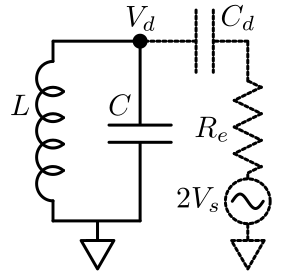
\includegraphics[width=4cm]{single_circuit_with_drive.pdf} 
\par\end{centering}
\caption{A parallel LC circuit. The main circuit is shown in solid line, while the driving circuit is shown in dotted line.}
\label{Fig:singleCircuit}
\end{figure}

